
%% Simplified structure file for IEEE style report

\documentclass[journal]{IEEEtran}

% *** CITATION PACKAGES ***
%
\usepackage{cite}
% cite.sty was written by Donald Arseneau
% V1.6 and later of IEEEtran pre-defines the format of the cite.sty package
% \cite{} output to follow that of the IEEE. Loading the cite package will
% result in citation numbers being automatically sorted and properly
% "compressed/ranged". e.g., [1], [9], [2], [7], [5], [6] without using
% cite.sty will become [1], [2], [5]--[7], [9] using cite.sty. cite.sty's
% \cite will automatically add leading space, if needed. Use cite.sty's
% noadjust option (cite.sty V3.8 and later) if you want to turn this off
% such as if a citation ever needs to be enclosed in parenthesis.
% cite.sty is already installed on most LaTeX systems. Be sure and use
% version 5.0 (2009-03-20) and later if using hyperref.sty.
% The latest version can be obtained at:
% http://www.ctan.org/pkg/cite
% The documentation is contained in the cite.sty file itself.


% *** GRAPHICS RELATED PACKAGES ***
%
\usepackage[pdftex]{graphicx}
% declare the path(s) where your graphic files are
% and their extensions so you won't have to specify these with
% every instance of \includegraphics
\graphicspath{{figs/}}
\DeclareGraphicsExtensions{.png}
% graphicx was written by David Carlisle and Sebastian Rahtz. It is
% required if you want graphics, photos, etc. graphicx.sty is already
% installed on most LaTeX systems. The latest version and documentation
% can be obtained at:
% http://www.ctan.org/pkg/graphicx
% Another good source of documentation is "Using Imported Graphics in
% LaTeX2e" by Keith Reckdahl which can be found at:
% http://www.ctan.org/pkg/epslatex
%
% latex, and pdflatex in dvi mode, support graphics in encapsulated
% postscript (.eps) format. pdflatex in pdf mode supports graphics
% in .pdf, .jpeg, .png and .mps (metapost) formats. Users should ensure
% that all non-photo figures use a vector format (.eps, .pdf, .mps) and
% not a bitmapped formats (.jpeg, .png). The IEEE frowns on bitmapped formats
% which can result in "jaggedy"/blurry rendering of lines and letters as
% well as large increases in file sizes.
%
% You can find documentation about the pdfTeX application at:
% http://www.tug.org/applications/pdftex


% *** MATH PACKAGES ***
%
%\usepackage{amsmath}
% A popular package from the American Mathematical Society that provides
% many useful and powerful commands for dealing with mathematics.
%
% Note that the amsmath package sets \interdisplaylinepenalty to 10000
% thus preventing page breaks from occurring within multiline equations. Use:
%\interdisplaylinepenalty=2500
% after loading amsmath to restore such page breaks as IEEEtran.cls normally
% does. amsmath.sty is already installed on most LaTeX systems. The latest
% version and documentation can be obtained at:
% http://www.ctan.org/pkg/amsmath

% *** SPECIALIZED LIST PACKAGES ***
%
%\usepackage{algorithmic}
% algorithmic.sty was written by Peter Williams and Rogerio Brito.
% This package provides an algorithmic environment fo describing algorithms.
% You can use the algorithmic environment in-text or within a figure
% environment to provide for a floating algorithm. Do NOT use the algorithm
% floating environment provided by algorithm.sty (by the same authors) or
% algorithm2e.sty (by Christophe Fiorio) as the IEEE does not use dedicated
% algorithm float types and packages that provide these will not provide
% correct IEEE style captions. The latest version and documentation of
% algorithmic.sty can be obtained at:
% http://www.ctan.org/pkg/algorithms
% Also of interest may be the (relatively newer and more customizable)
% algorithmicx.sty package by Szasz Janos:
% http://www.ctan.org/pkg/algorithmicx


% *** ALIGNMENT PACKAGES ***
%
\usepackage{array}
% Frank Mittelbach's and David Carlisle's array.sty patches and improves
% the standard LaTeX2e array and tabular environments to provide better
% appearance and additional user controls. As the default LaTeX2e table
% generation code is lacking to the point of almost being broken with
% respect to the quality of the end results, all users are strongly
% advised to use an enhanced (at the very least that provided by array.sty)
% set of table tools. array.sty is already installed on most systems. The
% latest version and documentation can be obtained at:
% http://www.ctan.org/pkg/array


% IEEEtran contains the IEEEeqnarray family of commands that can be used to
% generate multiline equations as well as matrices, tables, etc., of high
% quality.


% *** SUBFIGURE PACKAGES ***
\ifCLASSOPTIONcompsoc
  \usepackage[caption=false,font=normalsize,labelfont=sf,textfont=sf]{subfig}
\else
  \usepackage[caption=false,font=footnotesize]{subfig}
\fi
% subfig.sty, written by Steven Douglas Cochran, is the modern replacement
% for subfigure.sty, the latter of which is no longer maintained and is
% incompatible with some LaTeX packages including fixltx2e. However,
% subfig.sty requires and automatically loads Axel Sommerfeldt's caption.sty
% which will override IEEEtran.cls' handling of captions and this will result
% in non-IEEE style figure/table captions. To prevent this problem, be sure
% and invoke subfig.sty's "caption=false" package option (available since
% subfig.sty version 1.3, 2005/06/28) as this is will preserve IEEEtran.cls
% handling of captions.
% Note that the Computer Society format requires a larger sans serif font
% than the serif footnote size font used in traditional IEEE formatting
% and thus the need to invoke different subfig.sty package options depending
% on whether compsoc mode has been enabled.
%
% The latest version and documentation of subfig.sty can be obtained at:
% http://www.ctan.org/pkg/subfig



% *** Do not adjust lengths that control margins, column widths, etc. ***
% *** Do not use packages that alter fonts (such as pslatex).         ***
% There should be no need to do such things with IEEEtran.cls V1.6 and later.
% (Unless specifically asked to do so by the journal or conference you plan
% to submit to, of course. )

% required for degree symbol
\usepackage{gensymb}

% correct bad hyphenation here
\hyphenation{op-tical net-works semi-conduc-tor}


\begin{document}
%
% paper title
% Titles are generally capitalized except for words such as a, an, and, as,
% at, but, by, for, in, nor, of, on, or, the, to and up, which are usually
% not capitalized unless they are the first or last word of the title.
% Linebreaks \\ can be used within to get better formatting as desired.
% Do not put math or special symbols in the title.
\title{Investigating Tommy John Surgery With Machine Learning}
%
%
% author names
% note positions of commas and nonbreaking spaces ( ~ ) LaTeX will not break
% a structure at a ~ so this keeps an author's name from being broken across
% two lines.
\author{Nick~Seelert and Preston~Engstrom}
% note the % following the last name prevents an unwanted space from
% occurring between the last author name and the end of the author line

% The paper headers
\markboth{4P67 Machine Learning. Brock University. Friday, April 29, 2016}%
{Shell \MakeLowercase{\textit{et al.}}: Investigating Tommy John Surgery With Machine Learning}
% make the title area
\maketitle

% As a general rule, do not put math, special symbols or citations
% in the abstract or keywords.
\begin{abstract}
...
\end{abstract}

% Note that keywords are not normally used for peerreview papers.
% \begin{IEEEkeywords}
% IEEE, IEEEtran, journal, \LaTeX, paper, template.
% \end{IEEEkeywords}


%% BODY GOES HERE

\section {Introduction}
\IEEEPARstart{I}{n} 2015 the first ever prevalance study was conducted within all 30 Major League Baseball (MLB) organizations and reported 25\% of MLB pitchers had received TJS \cite{Conte2015}. Estimates previously had suggested the rate was much lower at 10\% \cite{Erickson2014}. The rapid rise in TJS occurance could be an increase in the number of injuries or simply be related to better understanding of the issue and injury data being more readily available allowing for more accurate measure \cite{Safran2005}. Regardless of the causes behind the numbers, the current risk is large with very little known about the risk factors. This makes it difficult for team doctors and pitchers to take the necessary preventative measures to avoid injury. At a minimum the injury is season ending, but it has the potential to alter pitchers career paths and have a financial impact on their teams.

It was reported that Major League Baseball's annual revenue for 2015 was \$9.5 billion \cite{ForbesMLB}. Some of the top grossing teams can afford to pay large multi-year contracts exceed \$200 million making players expensive assets to their teams. The teams investment can only be realized when the player is healthy and playing. It has been reported that elbow related injuries account for an average of 4451 days lost per MLB season \cite{Conte2015}. As such teams wish to mitigate their risk by investing in players with low risk exposure to long term injuries as well as winning performance measures.

Given the high prevalence of TJS observed along with the high monetary value of baseball players, it is of both medical and financial interest to investigate the risk factors associated with players requiring Tommy John surgery. By identifying risk factors it can help to develop preventative measures as well as reduce the risk exposure to teams regarding a player's health.

In this report we present an overview of the ulnar collateral ligament (UCL) and the damage that leads to Tommy John surgery. The problem of UCL injury and Tommy John surgery is then reviewed through previous published work in medical and academic journals. Based on this information present our own analysis of he problem using logistic regression and artifiial networks. Our results are discussed and compared with previous literature. We conclude with suggested future directions for furthering the understanding of the risks in baseball that lead to TJS.
\section {Background}

\subsection{Tommy John Surgery}

The surgery was first performed by Dr. Frank Jobe in 1974 on Tommy John due to irreversible damage done to the ulnar collateral ligament (UCL) in his pitching arm. As such UCL reconstruction surgery has become known as Tommy John surgery. The surgery replaces the damaged UCL in the pitching arm elbow of with a tendon from another body part. Originally the replacement tendon was taken from the forearm, however more recently doctors have favoured harvesting from the hamstring.

The degree to which requiring TJS affects a pitchers ability to return to play varies. However, several studies have reported between 67\% to 83\% of Major League Baseball (MLB) pitchers who underwent TJS returned to play at the same level \cite{Erickson2014} \cite{Cain2010} \cite{Makhni2014}. While the prospects for return are promising, it has been reported that it can take upwards of 16 months to return \cite{Makhni2014}. This is concerning to both the player and their team, especially if the are under a large contract.

It is widely believed by athletes and coaches that performance can actually improveme as a result of TJS \cite{Conte2015}. However, increases in performance after TJS can be related to strength gains during rehabilitation or mechanical improvements \cite{Cain2010}. The improvements may not even be real as the lower stats prior to the injury could be a result of impaired performance due to smaller injuries leading up to a full UCL tear. \cite{Makhni2014}. As such, there are no data to support prophylactic UCL reconstruction to improve performance or prevent injuries \cite{Erickson2014}

\subsection{Ulnar Collateral Ligament}

The UCL is a thick triangular ligament where each side of the triangle is a separate ligament (Figure \ref{fig:ucl_sketch}). The entire structure is located in the middle of the elbow toward the body. Of the three sub-ligaments, the anterior oblique ligament is the most important in terms of stress and forces. The anterior oblique ligament is commonly what is referred to as the UCL, as such we will also simply refer to the UCL.

\begin{figure}[ht]
    \centering
        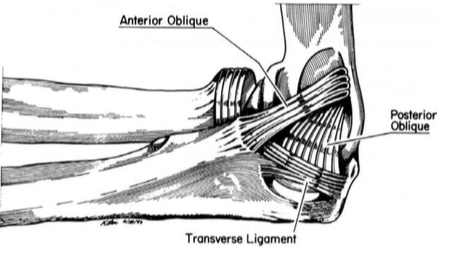
\includegraphics[width=0.45\textwidth]{ucl_sketch}
    \caption{Three sub ligaments make up the UCL. \cite{Safran2005}}
    \label{fig:ucl_sketch}
\end{figure}

\begin{figure}[hb]
    \centering
        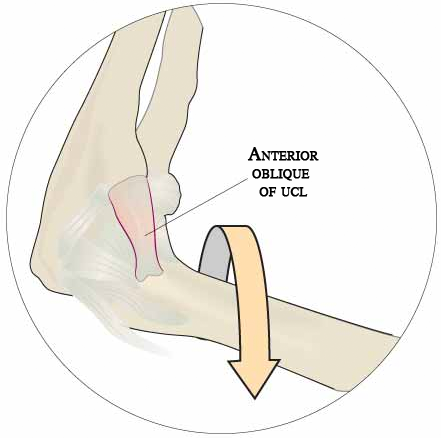
\includegraphics[width=0.3\textwidth]{ucl_torque}
    \caption{As arm rotates high valgus stress is generated on the UCL. \cite{NYTucl}}
    \label{fig:ucl_torque}
\end{figure}

Pitching generates high valgus and extension forces across the elbow \ref{fig:ucl_torque} during late cocking and acceleration phases. Stress is highest on the UCL when the elbow is flexed 90\degree and the shoulder is rotated away from the body \ref{fig:arm_pos} \cite{Fleisig2015}. At this point the anterior bundle of UCL is the primary restraint against valgus stress at the elbow. During this motion it is thought the vagus load approaches the maximum tensile strength of the UCL. It is therefore possible that a pitchers throwing elbow gradually leads to failure as a result of repeatedly being exposed to near-failure stresses \cite{Cain2010}

\begin{figure}[h]
    \centering
        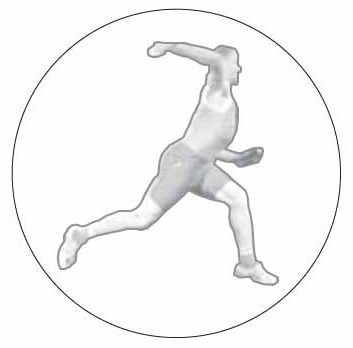
\includegraphics[width=0.3\textwidth]{arm_pos}
    \caption{Greatest valgus stress occurs during the late cocking phase of the pitchers throw. \cite{NYTucl}}
    \label{fig:arm_pos}
\end{figure}

Biomechanical studies have shown that moments of force on the shoulder and elbow as well as valgus torque are higher for fastballs than other pitches \cite{Keller2016}. This would suggest that pitchers that throw more fastballs could have an increased risk to UCL damage and thus increase chance of requiring TJS.

Given such a high prevlance of of TJS in professional baseball it is frustrating to all parties involved that diagnosing an UCL injury is difficult and likely not made until well after damage is done. One study suggested that diagnosis of UCL damage not made until an average of 6.4 months after symptoms began \cite{Cain2010}. One reason is can be so difficult to diagnose is that partial tearing of the UCL is likely indistinguishable from normal elbow laxity on examination. However, a player questionnaire reported that 96\% of players acknolwedged pain during the late cocking and acceleration phases of throwing \cite{Cain2010}. As such proper diagnosis may require a more qualitative analysis by team doctors with players.

\subsection{Risk Factors}

Many risk factors have been speculated including mechanics, pitch type, fatigue, overuse, velocity, and medical issues \cite{Keller2016} \cite{Fleisig2015}. However, proper investigation of the issue has been difficult. It has only been recently that the prevelance of TJS has been investigated and risk factors are only beginning to be uncovered \cite{Conte2015}. The ability to determine risk factors is also limited by studies being retrospective in nature. This limits the ability of researchers to determine changes in factors such as mechanics.

\subsection{Identifying Players at Risk}

\subsubsection{Common Statistics}

Several studies have made an attempt to find a relationship between declines in common pitcher statistics and the player requiring TJS. Comparing the pitchers statistics after returning from surgery hows shown a performance decrease, however the significance varies widely \cite{Makhni2014}. Also, several case-controlled studies failed to find a statistical difference between controls and injury pitchers \cite{Jiang2014} \cite{Erickson2014}.

It has been argued that common statistics like earned runs average (ERA), batting average against (BAA), and walks plus hits divided by innings pitched (WHIP) are not the best measures to consider when trying to investigate risk factors or predictors for TJS \cite{Gray2014}. This is due to the fact that these statistics are also affected by the ballpark the game is played in, the skill of the rest of the defense, luck, and several other factors. Factors more specific a pitchers performance would include fielding-independent pitching (FIP), pitch velocity, pitch type, movement, and other variables tracked for each pitch thrown by a pitcher.

\subsubsection{Pitch Specific Measures}

Every stadium in MLB has been equipped with the Sportvision PITCHf/X system. This system consists of 2 cameras located in the stands above home plate and first base. The purpose of these cameras is to track the flight of every pitch thrown and determine its position, velocity and acceleration \cite{Fast2010}. The system is paired with an MLB employee that records further information abouth the pitch such as strike, top and bottom of strike zone, etc.

Studies focusing directly on PITCHf/X data has also been varied. This could be largely due to the fact the classification algorithm used by the PITCHf/X system is constantly being tweaked so comparing data over multiple years can be counfounded by variation inherent in the system \cite{Fast2010}. In an attempt to overcome this several groups including the website http://brooksbaseball.net reviews all PITCHf/X data and manually reclassifies errors confirmed by their research.

While there can be a lot of noise present in the PITCHf/X data it is still useful to analyze. A study of 38 pitchers who had undergone TJS reported a small but significant decrease in the velocity of fastballs post injury \cite{Jiang2014}. However, a more recent study a larger sample size (83) failed to find a significant decrease in fastball velocity \cite{Keller2016}. Both studies were case-controlled and reported no significant difference in velocity between groups. However, it was reported that pitchers requiring TJS pitched a significantly higher percentage (7\%) of fastballs than controls. This suggests that the number of fastballs thrown is a risk factor but not the velocity of the pitch itself. \cite{Keller2016} Another study found decreases were observered in percentage of fastballs thrown and pitches in strike zone up to 2 years after surgery \cite{Makhni2014}. This may be related to changes in mechanics post surgery.

\subsubsection{Injury History}
A difficult set of factors to investigate in regards to players being at risk of UCL injury is previous injuries to the throwing arm, specifically the elbow. Difficulties are related to the available data on player injuries. Traditionally teams have preferred to hold exact details regarding their player's injuries, therefore data reported publically may not be accurate. However, in more recent years more data surrounding player injuries has become available and is making it easier to investigate.

One study looked at players being placed on the disabled list (DL), a public record of players removed from the teams active roster due to injury. The authors reported before surgery 74\% of players were placed on DL because of an injury to their throwing arm and of these 58\% were elbow related. After surgery 57\% of players were placed on DL because of an injury to their throwing arm, of which 26\% were an elbow injury \cite{Makhni2014}. This study was case-controlled and no significant difference was found between groups for total number of times placed on the DL for injuries related to the throwing arm. However, a higher number of of players requiring TJS went to DL specifically for elbow related injuries \cite{Makhni2014}.
\section{Methodology}

\subsection{Data Collection}

Data was collected and combined from several sources available online. Standard baseball statistics such as hits, walks, strike outs, etc. were collected from the Baseball Databank which is a publically maintained dataset of historical baseball data. Data was cloned from the Chadwick Baseball Databank GitHub repository \cite{ChadwickBD}. PITCHf/X and pitch count data was scraped from http://brooksbaseball.net using the XML package in RStudio 0.99.893. Players who underwent TJS between 2010-2015 were identified in the Baseball Injury Consultants private database. Access to this database was graciously provided to us by RockFence LLC. Data was obtained from this database using MySQLWorkbench 6.3.6 build 511 CE. Players were referenced by MLB media ID for PITCHf/X and Baseball IC data and by a Baseball Bureau reference ID for stats data obtained in the Baseball Databank. In order to cross reference the different ID types the Chadwick Baseball Bureau Register was used \cite{ChadwickR}. All data collectoin was conducted on a Macbook Pro with OS X El Capitain 10.11.4.

To construct the data set first a list of potential TJS case pitchers were obtained. This was done by identifying all pitchers labelled in the Baseball IC database as having undergone UCL Reconstruction. The year of surgery was considered as the index year for that pitcher. If a pitcher had multiple TJS only the first index year was selected. For all TJS cases PITCHf/X and statistical data was obtained for the index year and one year prior. Fielding Independent Pitching (FIP) calculations were made using the equation in Figure \ref{eq:fip}. The FIPs constants were collected from FanGraphs \cite{Fangraphs}. FIP is an attempt to give a measure similar to ERA but with more emphasis on plays that the pitcher has direct control over. This attempts to give a performance measure for the pitcher while removing the effect a luck and defense has on any individual pitcher \cite{FangraphsFIP}.

\begin{figure}[hb]
    \centering
        \[ FIP = \frac{13 * HR + 3 * (BB + HBP) - 2 * K}{IP} + FIPc\]
    \caption{FIP equation: HR is home runs, BB is walks, HBP is batters hit by pitch, K is strike outs, IP is innings pitched, and FIPc is the FIP constant. \cite{FangraphsFIP}}
    \label{eq:fip}
\end{figure}

\subsection{Input Selection}

Inputs were selected based on what was used in previous literature as well as taking into account critiques and improvements \cite{Gray2014}. From the statistical data, we selected home runs (HR), walks (BB), batters hit by pitch (HBP), strike outs (K), and innings pitched (IP). As stated above, these statistical variables were used to calculate the FIP score for each pitcher in an attempt to get a comparable performance statistic between pitchers. From the PITCHf/X data we selected average release speed (mph), max release speed (maxmph), horizontal movement (pfx\_x), vertical movement (pfx\_z), horizontal pitch location (hloc), vertical pitch location (vloc), and grooved pitches (bway) which are pitches straight down the center of home plate.

These variables were selected for each pitch type the player had used in the index year and year prior. Pitch counts were also collected for each pitch type a player had. The number of pitch types each pitcher has, therefore the number of variables with values could vary. To account for this we replaced any NA in pitchF/x and pitch count data with a 0 value. In total there were 156 input variables per player, however as previously stated many of these could be 0 due to pitchers not throwing all pitch types. One pitch type, screwballs, was only found in some control pitchers and was therefore dropped since no TJS pitcher had thrown any in their respective years.

\subsection{Control Selection}

Control pitchers were seleced with regard to TJS pitchers. For each index year between 2010-2015 groups were created where each control pitcher had data for that year and the year prior. For selection in analysis the TJS pitchers were first selected and then a control pitcher was selected from their respective bins based on TJS index year. We did no control for pitchers age or throwing arm, however birth year was included as an input.

\subsection{Data Analysis}
To analyze the data we conducted both foward and backward stepwise logistic regressions using the glm and step functions in RStudio 0.99.893. The selection process for the stepwise regressions with these functions is conducted using Akaike information criterion (AIC). The data was also run through the neural network package nnet 7.3-12 also in RStudio 0.99.893.







% if have a single appendix:
%\appendix[Proof of the Zonklar Equations]
% or
%\appendix  % for no appendix heading
% do not use \section anymore after \appendix, only \section*
% is possibly needed

% use appendices with more than one appendix
% then use \section to start each appendix
% you must declare a \section before using any
% \subsection or using \label (\appendices by itself
% starts a section numbered zero.)
%

%\appendices
%\section{Proof of the First Zonklar Equation}
%Appendix one text goes here.

% you can choose not to have a title for an appendix
% if you want by leaving the argument blank
%\section{}
%Appendix two text goes here.

% use section* for acknowledgment
%\section*{Acknowledgment}


% Can use something like this to put references on a page
% by themselves when using endfloat and the captionsoff option.
\ifCLASSOPTIONcaptionsoff
  \newpage
\fi
% trigger a \newpage just before the given reference
% number - used to balance the columns on the last page
% adjust value as needed - may need to be readjusted if
% the document is modified later
%\IEEEtriggeratref{8}
% The "triggered" command can be changed if desired:
%\IEEEtriggercmd{\enlargethispage{-5in}}

% references section
\bibliographystyle{IEEEtran}
\bibliography{references}

\end{document}